\documentclass[1p]{elsarticle_modified}
%\bibliographystyle{elsarticle-num}

%\usepackage[colorlinks]{hyperref}
%\usepackage{abbrmath_seonhwa} %\Abb, \Ascr, \Acal ,\Abf, \Afrak
\usepackage{amsfonts}
\usepackage{amssymb}
\usepackage{amsmath}
\usepackage{amsthm}
\usepackage{scalefnt}
\usepackage{amsbsy}
\usepackage{kotex}
\usepackage{caption}
\usepackage{subfig}
\usepackage{color}
\usepackage{graphicx}
\usepackage{xcolor} %% white, black, red, green, blue, cyan, magenta, yellow
\usepackage{float}
\usepackage{setspace}
\usepackage{hyperref}

\usepackage{tikz}
\usetikzlibrary{arrows}

\usepackage{multirow}
\usepackage{array} % fixed length table
\usepackage{hhline}

%%%%%%%%%%%%%%%%%%%%%
\makeatletter
\renewcommand*\env@matrix[1][\arraystretch]{%
	\edef\arraystretch{#1}%
	\hskip -\arraycolsep
	\let\@ifnextchar\new@ifnextchar
	\array{*\c@MaxMatrixCols c}}
\makeatother %https://tex.stackexchange.com/questions/14071/how-can-i-increase-the-line-spacing-in-a-matrix
%%%%%%%%%%%%%%%

\usepackage[normalem]{ulem}

\newcommand{\msout}[1]{\ifmmode\text{\sout{\ensuremath{#1}}}\else\sout{#1}\fi}
%SOURCE: \msout is \stkout macro in https://tex.stackexchange.com/questions/20609/strikeout-in-math-mode

\newcommand{\cancel}[1]{
	\ifmmode
	{\color{red}\msout{#1}}
	\else
	{\color{red}\sout{#1}}
	\fi
}

\newcommand{\add}[1]{
	{\color{blue}\uwave{#1}}
}

\newcommand{\replace}[2]{
	\ifmmode
	{\color{red}\msout{#1}}{\color{blue}\uwave{#2}}
	\else
	{\color{red}\sout{#1}}{\color{blue}\uwave{#2}}
	\fi
}

\newcommand{\Sol}{\mathcal{S}} %segment
\newcommand{\D}{D} %diagram
\newcommand{\A}{\mathcal{A}} %arc


%%%%%%%%%%%%%%%%%%%%%%%%%%%%%5 test

\def\sl{\operatorname{\textup{SL}}(2,\Cbb)}
\def\psl{\operatorname{\textup{PSL}}(2,\Cbb)}
\def\quan{\mkern 1mu \triangleright \mkern 1mu}

\theoremstyle{definition}
\newtheorem{thm}{Theorem}[section]
\newtheorem{prop}[thm]{Proposition}
\newtheorem{lem}[thm]{Lemma}
\newtheorem{ques}[thm]{Question}
\newtheorem{cor}[thm]{Corollary}
\newtheorem{defn}[thm]{Definition}
\newtheorem{exam}[thm]{Example}
\newtheorem{rmk}[thm]{Remark}
\newtheorem{alg}[thm]{Algorithm}

\newcommand{\I}{\sqrt{-1}}
\begin{document}

%\begin{frontmatter}
%
%\title{Boundary parabolic representations of knots up to 8 crossings}
%
%%% Group authors per affiliation:
%\author{Yunhi Cho} 
%\address{Department of Mathematics, University of Seoul, Seoul, Korea}
%\ead{yhcho@uos.ac.kr}
%
%
%\author{Seonhwa Kim} %\fnref{s_kim}}
%\address{Center for Geometry and Physics, Institute for Basic Science, Pohang, 37673, Korea}
%\ead{ryeona17@ibs.re.kr}
%
%\author{Hyuk Kim}
%\address{Department of Mathematical Sciences, Seoul National University, Seoul 08826, Korea}
%\ead{hyukkim@snu.ac.kr}
%
%\author{Seokbeom Yoon}
%\address{Department of Mathematical Sciences, Seoul National University, Seoul, 08826,  Korea}
%\ead{sbyoon15@snu.ac.kr}
%
%\begin{abstract}
%We find all boundary parabolic representation of knots up to 8 crossings.
%
%\end{abstract}
%\begin{keyword}
%    \MSC[2010] 57M25 
%\end{keyword}
%
%\end{frontmatter}

%\linenumbers
%\tableofcontents
%
\newcommand\colored[1]{\textcolor{white}{\rule[-0.35ex]{0.8em}{1.4ex}}\kern-0.8em\color{red} #1}%
%\newcommand\colored[1]{\textcolor{white}{ #1}\kern-2.17ex	\textcolor{white}{ #1}\kern-1.81ex	\textcolor{white}{ #1}\kern-2.15ex\color{red}#1	}

{\Large $\underline{12a_{0290}~(K12a_{0290})}$}

\setlength{\tabcolsep}{10pt}
\renewcommand{\arraystretch}{1.6}
\vspace{1cm}\begin{tabular}{m{100pt}>{\centering\arraybackslash}m{274pt}}
\multirow{5}{120pt}{
	\centering
	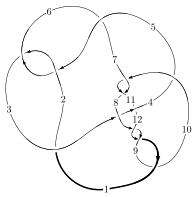
\includegraphics[width=112pt]{../../../GIT/diagram.site/Diagrams/png/1091_12a_0290.png}\\
\ \ \ A knot diagram\footnotemark}&
\allowdisplaybreaks
\textbf{Linearized knot diagam} \\
\cline{2-2}
 &
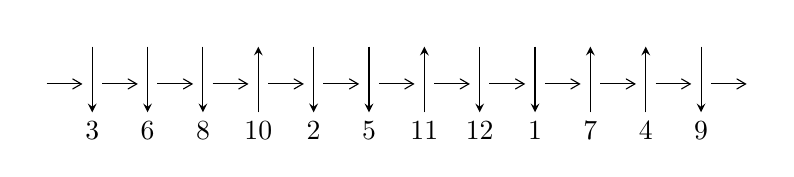
\begin{tikzpicture}[x=20pt, y=17pt]
	% nodes
	\node (C0) at (0, 0) {};
	\node (C1) at (1, 0) {};
	\node (C1U) at (1, +1) {};
	\node (C1D) at (1, -1) {3};

	\node (C2) at (2, 0) {};
	\node (C2U) at (2, +1) {};
	\node (C2D) at (2, -1) {6};

	\node (C3) at (3, 0) {};
	\node (C3U) at (3, +1) {};
	\node (C3D) at (3, -1) {8};

	\node (C4) at (4, 0) {};
	\node (C4U) at (4, +1) {};
	\node (C4D) at (4, -1) {10};

	\node (C5) at (5, 0) {};
	\node (C5U) at (5, +1) {};
	\node (C5D) at (5, -1) {2};

	\node (C6) at (6, 0) {};
	\node (C6U) at (6, +1) {};
	\node (C6D) at (6, -1) {5};

	\node (C7) at (7, 0) {};
	\node (C7U) at (7, +1) {};
	\node (C7D) at (7, -1) {11};

	\node (C8) at (8, 0) {};
	\node (C8U) at (8, +1) {};
	\node (C8D) at (8, -1) {12};

	\node (C9) at (9, 0) {};
	\node (C9U) at (9, +1) {};
	\node (C9D) at (9, -1) {1};

	\node (C10) at (10, 0) {};
	\node (C10U) at (10, +1) {};
	\node (C10D) at (10, -1) {7};

	\node (C11) at (11, 0) {};
	\node (C11U) at (11, +1) {};
	\node (C11D) at (11, -1) {4};

	\node (C12) at (12, 0) {};
	\node (C12U) at (12, +1) {};
	\node (C12D) at (12, -1) {9};
	\node (C13) at (13, 0) {};

	% arrows
	\draw[->,>={angle 60}]
	(C0) edge (C1) (C1) edge (C2) (C2) edge (C3) (C3) edge (C4) (C4) edge (C5) (C5) edge (C6) (C6) edge (C7) (C7) edge (C8) (C8) edge (C9) (C9) edge (C10) (C10) edge (C11) (C11) edge (C12) (C12) edge (C13) ;	\draw[->,>=stealth]
	(C1U) edge (C1D) (C2U) edge (C2D) (C3U) edge (C3D) (C4D) edge (C4U) (C5U) edge (C5D) (C6U) edge (C6D) (C7D) edge (C7U) (C8U) edge (C8D) (C9U) edge (C9D) (C10D) edge (C10U) (C11D) edge (C11U) (C12U) edge (C12D) ;
	\end{tikzpicture} \\
\hhline{~~} \\& 
\textbf{Solving Sequence} \\ \cline{2-2} 
 &
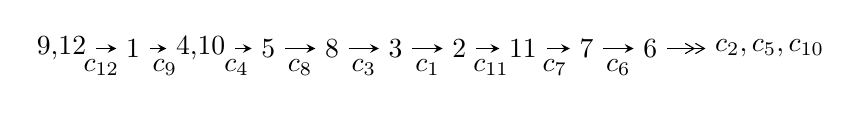
\begin{tikzpicture}[x=23pt, y=7pt]
	% node
	\node (A0) at (-1/8, 0) {9,12};
	\node (A1) at (1, 0) {1};
	\node (A2) at (33/16, 0) {4,10};
	\node (A3) at (25/8, 0) {5};
	\node (A4) at (33/8, 0) {8};
	\node (A5) at (41/8, 0) {3};
	\node (A6) at (49/8, 0) {2};
	\node (A7) at (57/8, 0) {11};
	\node (A8) at (65/8, 0) {7};
	\node (A9) at (73/8, 0) {6};
	\node (C1) at (1/2, -1) {$c_{12}$};
	\node (C2) at (3/2, -1) {$c_{9}$};
	\node (C3) at (21/8, -1) {$c_{4}$};
	\node (C4) at (29/8, -1) {$c_{8}$};
	\node (C5) at (37/8, -1) {$c_{3}$};
	\node (C6) at (45/8, -1) {$c_{1}$};
	\node (C7) at (53/8, -1) {$c_{11}$};
	\node (C8) at (61/8, -1) {$c_{7}$};
	\node (C9) at (69/8, -1) {$c_{6}$};
	\node (A10) at (11, 0) {$c_{2},c_{5},c_{10}$};

	% edge
	\draw[->,>=stealth]	
	(A0) edge (A1) (A1) edge (A2) (A2) edge (A3) (A3) edge (A4) (A4) edge (A5) (A5) edge (A6) (A6) edge (A7) (A7) edge (A8) (A8) edge (A9) ;
	\draw[->>,>={angle 60}]	
	(A9) edge (A10);
\end{tikzpicture} \\ 

\end{tabular} \\

\footnotetext{
The image of knot diagram is generated by the software ``\textbf{Draw programme}" developed by Andrew Bartholomew(\url{http://www.layer8.co.uk/maths/draw/index.htm\#Running-draw}), where we modified some parts for our purpose(\url{https://github.com/CATsTAILs/LinksPainter}).
}\phantom \\ \newline 
\centering \textbf{Ideals for irreducible components\footnotemark of $X_{\text{par}}$} 
 
\begin{align*}
I^u_{1}&=\langle 
1.57175\times10^{132} u^{87}+1.72314\times10^{133} u^{86}+\cdots+9.74392\times10^{132} b+5.16952\times10^{132},\\
\phantom{I^u_{1}}&\phantom{= \langle  }6.77338\times10^{132} u^{87}+6.23699\times10^{133} u^{86}+\cdots+9.74392\times10^{132} a-1.46464\times10^{132},\;u^{88}+7 u^{87}+\cdots+6 u-2\rangle \\
I^u_{2}&=\langle 
b+1,\;2 a- u,\;u^2-2\rangle \\
\\
I^v_{1}&=\langle 
a,\;b-1,\;v+1\rangle \\
\end{align*}
\raggedright * 3 irreducible components of $\dim_{\mathbb{C}}=0$, with total 91 representations.\\
\footnotetext{All coefficients of polynomials are rational numbers. But the coefficients are sometimes approximated in decimal forms when there is not enough margin.}
\newpage
\renewcommand{\arraystretch}{1}
\centering \section*{I. $I^u_{1}= \langle 1.57\times10^{132} u^{87}+1.72\times10^{133} u^{86}+\cdots+9.74\times10^{132} b+5.17\times10^{132},\;6.77\times10^{132} u^{87}+6.24\times10^{133} u^{86}+\cdots+9.74\times10^{132} a-1.46\times10^{132},\;u^{88}+7 u^{87}+\cdots+6 u-2 \rangle$}
\flushleft \textbf{(i) Arc colorings}\\
\begin{tabular}{m{7pt} m{180pt} m{7pt} m{180pt} }
\flushright $a_{9}=$&$\begin{pmatrix}0\\u\end{pmatrix}$ \\
\flushright $a_{12}=$&$\begin{pmatrix}1\\0\end{pmatrix}$ \\
\flushright $a_{1}=$&$\begin{pmatrix}1\\u^2\end{pmatrix}$ \\
\flushright $a_{4}=$&$\begin{pmatrix}-0.695139 u^{87}-6.40091 u^{86}+\cdots-9.75797 u+0.150314\\-0.161305 u^{87}-1.76843 u^{86}+\cdots+3.10463 u-0.530538\end{pmatrix}$ \\
\flushright $a_{10}=$&$\begin{pmatrix}- u\\- u^3+u\end{pmatrix}$ \\
\flushright $a_{5}=$&$\begin{pmatrix}0.671807 u^{87}+4.32742 u^{86}+\cdots-10.5704 u+1.48658\\1.00155 u^{87}+7.58488 u^{86}+\cdots-0.307323 u+0.452612\end{pmatrix}$ \\
\flushright $a_{8}=$&$\begin{pmatrix}u\\u\end{pmatrix}$ \\
\flushright $a_{3}=$&$\begin{pmatrix}1.42894 u^{87}+10.3800 u^{86}+\cdots-14.0642 u+1.94160\\1.96278 u^{87}+15.0125 u^{86}+\cdots-1.20156 u+1.26075\end{pmatrix}$ \\
\flushright $a_{2}=$&$\begin{pmatrix}1.09670 u^{87}+5.26132 u^{86}+\cdots+11.8149 u-1.97450\\0.586103 u^{87}+0.737960 u^{86}+\cdots+12.2825 u-4.91592\end{pmatrix}$ \\
\flushright $a_{11}=$&$\begin{pmatrix}-0.555259 u^{87}-2.94764 u^{86}+\cdots-12.5540 u+2.00113\\-0.932863 u^{87}-5.26350 u^{86}+\cdots-0.350537 u-0.580112\end{pmatrix}$ \\
\flushright $a_{7}=$&$\begin{pmatrix}0.555259 u^{87}+2.94764 u^{86}+\cdots+12.5540 u-2.00113\\0.445220 u^{87}+2.37310 u^{86}+\cdots+6.39498 u-2.45844\end{pmatrix}$ \\
\flushright $a_{6}=$&$\begin{pmatrix}-0.986580 u^{87}-5.40335 u^{86}+\cdots+0.0651781 u+0.914542\\-0.613296 u^{87}-1.77328 u^{86}+\cdots-8.33907 u+2.76232\end{pmatrix}$\\&\end{tabular}
\flushleft \textbf{(ii) Obstruction class $= -1$}\\~\\
\flushleft \textbf{(iii) Cusp Shapes $= -4.29383 u^{87}-32.7289 u^{86}+\cdots-26.3353 u+8.92622$}\\~\\
\newpage\renewcommand{\arraystretch}{1}
\flushleft \textbf{(iv) u-Polynomials at the component}\newline \\
\begin{tabular}{m{50pt}|m{274pt}}
Crossings & \hspace{64pt}u-Polynomials at each crossing \\
\hline $$\begin{aligned}c_{1},c_{6}\end{aligned}$$&$\begin{aligned}
&u^{88}+28 u^{87}+\cdots-66 u+1
\end{aligned}$\\
\hline $$\begin{aligned}c_{2},c_{5}\end{aligned}$$&$\begin{aligned}
&u^{88}+4 u^{87}+\cdots+2 u+1
\end{aligned}$\\
\hline $$\begin{aligned}c_{3}\end{aligned}$$&$\begin{aligned}
&u^{88}-26 u^{87}+\cdots+4 u+1
\end{aligned}$\\
\hline $$\begin{aligned}c_{4}\end{aligned}$$&$\begin{aligned}
&u^{88}+32 u^{87}+\cdots-17646936 u-2939221
\end{aligned}$\\
\hline $$\begin{aligned}c_{7},c_{10}\end{aligned}$$&$\begin{aligned}
&u^{88}-2 u^{87}+\cdots-34 u-1
\end{aligned}$\\
\hline $$\begin{aligned}c_{8},c_{9},c_{12}\end{aligned}$$&$\begin{aligned}
&u^{88}+7 u^{87}+\cdots+6 u-2
\end{aligned}$\\
\hline $$\begin{aligned}c_{11}\end{aligned}$$&$\begin{aligned}
&u^{88}-4 u^{87}+\cdots+10 u-1
\end{aligned}$\\
\hline
\end{tabular}\\~\\
\newpage\renewcommand{\arraystretch}{1}
\flushleft \textbf{(v) Riley Polynomials at the component}\newline \\
\begin{tabular}{m{50pt}|m{274pt}}
Crossings & \hspace{64pt}Riley Polynomials at each crossing \\
\hline $$\begin{aligned}c_{1},c_{6}\end{aligned}$$&$\begin{aligned}
&y^{88}+68 y^{87}+\cdots-1966 y+1
\end{aligned}$\\
\hline $$\begin{aligned}c_{2},c_{5}\end{aligned}$$&$\begin{aligned}
&y^{88}-28 y^{87}+\cdots+66 y+1
\end{aligned}$\\
\hline $$\begin{aligned}c_{3}\end{aligned}$$&$\begin{aligned}
&y^{88}-512 y^{87}+\cdots-758 y+1
\end{aligned}$\\
\hline $$\begin{aligned}c_{4}\end{aligned}$$&$\begin{aligned}
&y^{88}-588 y^{87}+\cdots-154392187987162 y+8639020086841
\end{aligned}$\\
\hline $$\begin{aligned}c_{7},c_{10}\end{aligned}$$&$\begin{aligned}
&y^{88}-68 y^{87}+\cdots-630 y+1
\end{aligned}$\\
\hline $$\begin{aligned}c_{8},c_{9},c_{12}\end{aligned}$$&$\begin{aligned}
&y^{88}-85 y^{87}+\cdots+28 y+4
\end{aligned}$\\
\hline $$\begin{aligned}c_{11}\end{aligned}$$&$\begin{aligned}
&y^{88}+4 y^{87}+\cdots-70 y+1
\end{aligned}$\\
\hline
\end{tabular}\\~\\
\newpage\flushleft \textbf{(vi) Complex Volumes and Cusp Shapes}
$$\begin{array}{c|c|c}  
\text{Solutions to }I^u_{1}& \I (\text{vol} + \sqrt{-1}CS) & \text{Cusp shape}\\
 \hline 
\begin{aligned}
u &= \phantom{-}0.495208 + 0.877151 I \\
a &= \phantom{-}0.411455 + 0.753705 I \\
b &= -1.015090 + 0.935019 I\end{aligned}
 & \phantom{-}7.6509 - 12.9288 I & \phantom{-0.000000 } 0 \\ \hline\begin{aligned}
u &= \phantom{-}0.495208 - 0.877151 I \\
a &= \phantom{-}0.411455 - 0.753705 I \\
b &= -1.015090 - 0.935019 I\end{aligned}
 & \phantom{-}7.6509 + 12.9288 I & \phantom{-0.000000 } 0 \\ \hline\begin{aligned}
u &= -0.281152 + 0.967426 I \\
a &= -0.291698 + 0.134353 I \\
b &= \phantom{-}0.472094 + 0.654902 I\end{aligned}
 & \phantom{-}2.59156 + 1.21821 I & \phantom{-0.000000 } 0 \\ \hline\begin{aligned}
u &= -0.281152 - 0.967426 I \\
a &= -0.291698 - 0.134353 I \\
b &= \phantom{-}0.472094 - 0.654902 I\end{aligned}
 & \phantom{-}2.59156 - 1.21821 I & \phantom{-0.000000 } 0 \\ \hline\begin{aligned}
u &= \phantom{-}0.444403 + 0.862629 I \\
a &= -0.409808 - 0.736494 I \\
b &= \phantom{-}1.025420 - 0.939996 I\end{aligned}
 & \phantom{-}8.42853 - 6.77648 I & \phantom{-0.000000 } 0 \\ \hline\begin{aligned}
u &= \phantom{-}0.444403 - 0.862629 I \\
a &= -0.409808 + 0.736494 I \\
b &= \phantom{-}1.025420 + 0.939996 I\end{aligned}
 & \phantom{-}8.42853 + 6.77648 I & \phantom{-0.000000 } 0 \\ \hline\begin{aligned}
u &= -0.612876 + 0.708935 I \\
a &= \phantom{-}0.346947 - 0.372276 I \\
b &= -0.395815 - 0.656615 I\end{aligned}
 & -2.85481 + 2.65153 I & \phantom{-0.000000 } 0 \\ \hline\begin{aligned}
u &= -0.612876 - 0.708935 I \\
a &= \phantom{-}0.346947 + 0.372276 I \\
b &= -0.395815 + 0.656615 I\end{aligned}
 & -2.85481 - 2.65153 I & \phantom{-0.000000 } 0 \\ \hline\begin{aligned}
u &= -0.386006 + 1.003120 I \\
a &= \phantom{-}0.270380 - 0.196109 I \\
b &= -0.456111 - 0.671602 I\end{aligned}
 & \phantom{-}2.15335 + 6.83792 I & \phantom{-0.000000 } 0 \\ \hline\begin{aligned}
u &= -0.386006 - 1.003120 I \\
a &= \phantom{-}0.270380 + 0.196109 I \\
b &= -0.456111 + 0.671602 I\end{aligned}
 & \phantom{-}2.15335 - 6.83792 I & \phantom{-0.000000 } 0\\
 \hline 
 \end{array}$$\newpage$$\begin{array}{c|c|c}  
\text{Solutions to }I^u_{1}& \I (\text{vol} + \sqrt{-1}CS) & \text{Cusp shape}\\
 \hline 
\begin{aligned}
u &= \phantom{-}0.752047 + 0.815149 I \\
a &= -0.563170 + 0.131031 I \\
b &= -0.816592 - 0.610525 I\end{aligned}
 & \phantom{-}7.57889 + 1.20760 I & \phantom{-0.000000 } 0 \\ \hline\begin{aligned}
u &= \phantom{-}0.752047 - 0.815149 I \\
a &= -0.563170 - 0.131031 I \\
b &= -0.816592 + 0.610525 I\end{aligned}
 & \phantom{-}7.57889 - 1.20760 I & \phantom{-0.000000 } 0 \\ \hline\begin{aligned}
u &= \phantom{-}0.704958 + 0.876898 I \\
a &= \phantom{-}0.479501 - 0.130087 I \\
b &= \phantom{-}0.785629 + 0.624303 I\end{aligned}
 & \phantom{-}7.10312 + 7.15665 I & \phantom{-0.000000 } 0 \\ \hline\begin{aligned}
u &= \phantom{-}0.704958 - 0.876898 I \\
a &= \phantom{-}0.479501 + 0.130087 I \\
b &= \phantom{-}0.785629 - 0.624303 I\end{aligned}
 & \phantom{-}7.10312 - 7.15665 I & \phantom{-0.000000 } 0 \\ \hline\begin{aligned}
u &= -1.174970 + 0.061073 I \\
a &= -0.00514 - 2.91113 I \\
b &= -0.18951 - 1.68930 I\end{aligned}
 & \phantom{-}5.02727 + 3.33290 I & \phantom{-0.000000 } 0 \\ \hline\begin{aligned}
u &= -1.174970 - 0.061073 I \\
a &= -0.00514 + 2.91113 I \\
b &= -0.18951 + 1.68930 I\end{aligned}
 & \phantom{-}5.02727 - 3.33290 I & \phantom{-0.000000 } 0 \\ \hline\begin{aligned}
u &= \phantom{-}0.508152 + 0.646507 I \\
a &= \phantom{-}0.502496 + 0.724043 I \\
b &= -1.051760 + 0.875815 I\end{aligned}
 & \phantom{-}0.64818 - 7.68033 I & -4.00000 + 9.27908 I \\ \hline\begin{aligned}
u &= \phantom{-}0.508152 - 0.646507 I \\
a &= \phantom{-}0.502496 - 0.724043 I \\
b &= -1.051760 - 0.875815 I\end{aligned}
 & \phantom{-}0.64818 + 7.68033 I & -4.00000 - 9.27908 I \\ \hline\begin{aligned}
u &= \phantom{-}0.385530 + 0.718019 I \\
a &= \phantom{-}0.210598 - 0.555538 I \\
b &= \phantom{-}0.667580 + 0.521758 I\end{aligned}
 & \phantom{-}1.01440 + 3.28538 I & -4.00000 - 6.83921 I \\ \hline\begin{aligned}
u &= \phantom{-}0.385530 - 0.718019 I \\
a &= \phantom{-}0.210598 + 0.555538 I \\
b &= \phantom{-}0.667580 - 0.521758 I\end{aligned}
 & \phantom{-}1.01440 - 3.28538 I & -4.00000 + 6.83921 I\\
 \hline 
 \end{array}$$\newpage$$\begin{array}{c|c|c}  
\text{Solutions to }I^u_{1}& \I (\text{vol} + \sqrt{-1}CS) & \text{Cusp shape}\\
 \hline 
\begin{aligned}
u &= \phantom{-}1.271860 + 0.189390 I \\
a &= -1.57244 - 0.54471 I \\
b &= -1.62915 - 0.67700 I\end{aligned}
 & \phantom{-}3.80798 - 2.18851 I & \phantom{-0.000000 } 0 \\ \hline\begin{aligned}
u &= \phantom{-}1.271860 - 0.189390 I \\
a &= -1.57244 + 0.54471 I \\
b &= -1.62915 + 0.67700 I\end{aligned}
 & \phantom{-}3.80798 + 2.18851 I & \phantom{-0.000000 } 0 \\ \hline\begin{aligned}
u &= \phantom{-}1.30786\phantom{ +0.000000I} \\
a &= \phantom{-}2.40716\phantom{ +0.000000I} \\
b &= \phantom{-}2.44403\phantom{ +0.000000I}\end{aligned}
 & -3.20868\phantom{ +0.000000I} & \phantom{-0.000000 } 0 \\ \hline\begin{aligned}
u &= \phantom{-}0.312791 + 0.615361 I \\
a &= -0.457552 - 0.634789 I \\
b &= \phantom{-}1.12009 - 0.93330 I\end{aligned}
 & \phantom{-}3.95546 - 4.04673 I & \phantom{-}2.71866 + 5.71962 I \\ \hline\begin{aligned}
u &= \phantom{-}0.312791 - 0.615361 I \\
a &= -0.457552 + 0.634789 I \\
b &= \phantom{-}1.12009 + 0.93330 I\end{aligned}
 & \phantom{-}3.95546 + 4.04673 I & \phantom{-}2.71866 - 5.71962 I \\ \hline\begin{aligned}
u &= \phantom{-}0.578857 + 0.359329 I \\
a &= -1.23689 + 0.76115 I \\
b &= -0.804602 - 0.317174 I\end{aligned}
 & \phantom{-}2.95975 + 0.61087 I & \phantom{-}0.98547 + 2.25403 I \\ \hline\begin{aligned}
u &= \phantom{-}0.578857 - 0.359329 I \\
a &= -1.23689 - 0.76115 I \\
b &= -0.804602 + 0.317174 I\end{aligned}
 & \phantom{-}2.95975 - 0.61087 I & \phantom{-}0.98547 - 2.25403 I \\ \hline\begin{aligned}
u &= \phantom{-}1.328780 + 0.000300 I \\
a &= \phantom{-}0.44226 + 2.75769 I \\
b &= -0.128258 + 0.645110 I\end{aligned}
 & -0.20961 - 2.93911 I & \phantom{-0.000000 } 0 \\ \hline\begin{aligned}
u &= \phantom{-}1.328780 - 0.000300 I \\
a &= \phantom{-}0.44226 - 2.75769 I \\
b &= -0.128258 - 0.645110 I\end{aligned}
 & -0.20961 + 2.93911 I & \phantom{-0.000000 } 0 \\ \hline\begin{aligned}
u &= -1.325330 + 0.124435 I \\
a &= -0.037394 + 0.440662 I \\
b &= -0.911325 + 0.455131 I\end{aligned}
 & -1.304860 + 0.085633 I & \phantom{-0.000000 } 0\\
 \hline 
 \end{array}$$\newpage$$\begin{array}{c|c|c}  
\text{Solutions to }I^u_{1}& \I (\text{vol} + \sqrt{-1}CS) & \text{Cusp shape}\\
 \hline 
\begin{aligned}
u &= -1.325330 - 0.124435 I \\
a &= -0.037394 - 0.440662 I \\
b &= -0.911325 - 0.455131 I\end{aligned}
 & -1.304860 - 0.085633 I & \phantom{-0.000000 } 0 \\ \hline\begin{aligned}
u &= \phantom{-}1.355190 + 0.192450 I \\
a &= \phantom{-}1.51658 + 0.83209 I \\
b &= \phantom{-}1.63713 + 0.93870 I\end{aligned}
 & \phantom{-}2.27442 - 8.32858 I & \phantom{-0.000000 } 0 \\ \hline\begin{aligned}
u &= \phantom{-}1.355190 - 0.192450 I \\
a &= \phantom{-}1.51658 - 0.83209 I \\
b &= \phantom{-}1.63713 - 0.93870 I\end{aligned}
 & \phantom{-}2.27442 + 8.32858 I & \phantom{-0.000000 } 0 \\ \hline\begin{aligned}
u &= -1.368320 + 0.067286 I \\
a &= \phantom{-}0.466668 - 0.523121 I \\
b &= -0.324757 - 0.265684 I\end{aligned}
 & -3.14744 + 0.11184 I & \phantom{-0.000000 } 0 \\ \hline\begin{aligned}
u &= -1.368320 - 0.067286 I \\
a &= \phantom{-}0.466668 + 0.523121 I \\
b &= -0.324757 + 0.265684 I\end{aligned}
 & -3.14744 - 0.11184 I & \phantom{-0.000000 } 0 \\ \hline\begin{aligned}
u &= \phantom{-}1.383300 + 0.016208 I \\
a &= -1.70570 + 5.79045 I \\
b &= \phantom{-}0.082745 + 0.273472 I\end{aligned}
 & -0.20747 - 2.85455 I & \phantom{-0.000000 } 0 \\ \hline\begin{aligned}
u &= \phantom{-}1.383300 - 0.016208 I \\
a &= -1.70570 - 5.79045 I \\
b &= \phantom{-}0.082745 - 0.273472 I\end{aligned}
 & -0.20747 + 2.85455 I & \phantom{-0.000000 } 0 \\ \hline\begin{aligned}
u &= -0.088016 + 0.606452 I \\
a &= -0.304643 - 0.577626 I \\
b &= \phantom{-}1.05284 - 1.12404 I\end{aligned}
 & \phantom{-}7.98061 - 0.72495 I & \phantom{-}5.07684 + 0.22833 I \\ \hline\begin{aligned}
u &= -0.088016 - 0.606452 I \\
a &= -0.304643 + 0.577626 I \\
b &= \phantom{-}1.05284 + 1.12404 I\end{aligned}
 & \phantom{-}7.98061 + 0.72495 I & \phantom{-}5.07684 - 0.22833 I \\ \hline\begin{aligned}
u &= -1.386200 + 0.131809 I \\
a &= \phantom{-}0.141767 - 0.467812 I \\
b &= \phantom{-}1.028830 - 0.460792 I\end{aligned}
 & -2.12556 + 5.58667 I & \phantom{-0.000000 } 0\\
 \hline 
 \end{array}$$\newpage$$\begin{array}{c|c|c}  
\text{Solutions to }I^u_{1}& \I (\text{vol} + \sqrt{-1}CS) & \text{Cusp shape}\\
 \hline 
\begin{aligned}
u &= -1.386200 - 0.131809 I \\
a &= \phantom{-}0.141767 + 0.467812 I \\
b &= \phantom{-}1.028830 + 0.460792 I\end{aligned}
 & -2.12556 - 5.58667 I & \phantom{-0.000000 } 0 \\ \hline\begin{aligned}
u &= -0.187730 + 0.577154 I \\
a &= \phantom{-}0.271356 + 0.574587 I \\
b &= -0.99826 + 1.15457 I\end{aligned}
 & \phantom{-}7.13319 + 5.55022 I & \phantom{-}3.18440 - 6.17368 I \\ \hline\begin{aligned}
u &= -0.187730 - 0.577154 I \\
a &= \phantom{-}0.271356 - 0.574587 I \\
b &= -0.99826 - 1.15457 I\end{aligned}
 & \phantom{-}7.13319 - 5.55022 I & \phantom{-}3.18440 + 6.17368 I \\ \hline\begin{aligned}
u &= -0.603442 + 0.033860 I \\
a &= \phantom{-}0.196407 - 0.659993 I \\
b &= -0.346103 - 0.850656 I\end{aligned}
 & -1.47881 - 1.50127 I & -9.75731 + 4.59132 I \\ \hline\begin{aligned}
u &= -0.603442 - 0.033860 I \\
a &= \phantom{-}0.196407 + 0.659993 I \\
b &= -0.346103 + 0.850656 I\end{aligned}
 & -1.47881 + 1.50127 I & -9.75731 - 4.59132 I \\ \hline\begin{aligned}
u &= -1.40622\phantom{ +0.000000I} \\
a &= \phantom{-}0.301859\phantom{ +0.000000I} \\
b &= \phantom{-}1.14642\phantom{ +0.000000I}\end{aligned}
 & -6.56478\phantom{ +0.000000I} & \phantom{-0.000000 } 0 \\ \hline\begin{aligned}
u &= \phantom{-}1.41892\phantom{ +0.000000I} \\
a &= -17.7637\phantom{ +0.000000I} \\
b &= \phantom{-}0.0959723\phantom{ +0.000000I}\end{aligned}
 & -4.41271\phantom{ +0.000000I} & \phantom{-0.000000 } 0 \\ \hline\begin{aligned}
u &= -1.41358 + 0.13459 I \\
a &= \phantom{-}0.70257 + 2.34250 I \\
b &= \phantom{-}1.28835 + 1.74535 I\end{aligned}
 & -5.42809 + 2.53490 I & \phantom{-0.000000 } 0 \\ \hline\begin{aligned}
u &= -1.41358 - 0.13459 I \\
a &= \phantom{-}0.70257 - 2.34250 I \\
b &= \phantom{-}1.28835 - 1.74535 I\end{aligned}
 & -5.42809 - 2.53490 I & \phantom{-0.000000 } 0 \\ \hline\begin{aligned}
u &= -1.32882 + 0.54023 I \\
a &= \phantom{-}0.185595 - 0.497662 I \\
b &= -0.302391 - 0.629403 I\end{aligned}
 & -0.626564 - 0.632614 I & \phantom{-0.000000 } 0\\
 \hline 
 \end{array}$$\newpage$$\begin{array}{c|c|c}  
\text{Solutions to }I^u_{1}& \I (\text{vol} + \sqrt{-1}CS) & \text{Cusp shape}\\
 \hline 
\begin{aligned}
u &= -1.32882 - 0.54023 I \\
a &= \phantom{-}0.185595 + 0.497662 I \\
b &= -0.302391 + 0.629403 I\end{aligned}
 & -0.626564 + 0.632614 I & \phantom{-0.000000 } 0 \\ \hline\begin{aligned}
u &= -1.42235 + 0.21993 I \\
a &= -0.32909 - 2.17060 I \\
b &= -1.08443 - 1.47205 I\end{aligned}
 & -1.60919 + 7.07285 I & \phantom{-0.000000 } 0 \\ \hline\begin{aligned}
u &= -1.42235 - 0.21993 I \\
a &= -0.32909 + 2.17060 I \\
b &= -1.08443 + 1.47205 I\end{aligned}
 & -1.60919 - 7.07285 I & \phantom{-0.000000 } 0 \\ \hline\begin{aligned}
u &= \phantom{-}1.43564 + 0.16847 I \\
a &= \phantom{-}0.16509 + 1.64037 I \\
b &= -0.549615 + 1.090380 I\end{aligned}
 & -5.77675 - 3.38269 I & \phantom{-0.000000 } 0 \\ \hline\begin{aligned}
u &= \phantom{-}1.43564 - 0.16847 I \\
a &= \phantom{-}0.16509 - 1.64037 I \\
b &= -0.549615 - 1.090380 I\end{aligned}
 & -5.77675 + 3.38269 I & \phantom{-0.000000 } 0 \\ \hline\begin{aligned}
u &= -0.289821 + 0.442277 I \\
a &= -0.750944 + 0.488100 I \\
b &= \phantom{-}0.357107 + 0.565907 I\end{aligned}
 & -0.130405 + 1.105450 I & -2.09917 - 6.01174 I \\ \hline\begin{aligned}
u &= -0.289821 - 0.442277 I \\
a &= -0.750944 - 0.488100 I \\
b &= \phantom{-}0.357107 - 0.565907 I\end{aligned}
 & -0.130405 - 1.105450 I & -2.09917 + 6.01174 I \\ \hline\begin{aligned}
u &= -0.511705 + 0.082203 I \\
a &= -0.71931 + 4.95483 I \\
b &= \phantom{-}0.076717 + 0.762273 I\end{aligned}
 & \phantom{-}5.46748 - 2.98633 I & -9.54273 + 0.07763 I \\ \hline\begin{aligned}
u &= -0.511705 - 0.082203 I \\
a &= -0.71931 - 4.95483 I \\
b &= \phantom{-}0.076717 - 0.762273 I\end{aligned}
 & \phantom{-}5.46748 + 2.98633 I & -9.54273 - 0.07763 I \\ \hline\begin{aligned}
u &= \phantom{-}1.49176 + 0.09347 I \\
a &= \phantom{-}0.04638 - 1.73361 I \\
b &= \phantom{-}0.526261 - 1.275590 I\end{aligned}
 & -8.28685 + 0.58022 I & \phantom{-0.000000 } 0\\
 \hline 
 \end{array}$$\newpage$$\begin{array}{c|c|c}  
\text{Solutions to }I^u_{1}& \I (\text{vol} + \sqrt{-1}CS) & \text{Cusp shape}\\
 \hline 
\begin{aligned}
u &= \phantom{-}1.49176 - 0.09347 I \\
a &= \phantom{-}0.04638 + 1.73361 I \\
b &= \phantom{-}0.526261 + 1.275590 I\end{aligned}
 & -8.28685 - 0.58022 I & \phantom{-0.000000 } 0 \\ \hline\begin{aligned}
u &= \phantom{-}1.45601 + 0.33912 I \\
a &= \phantom{-}0.213193 + 1.364660 I \\
b &= -0.705900 + 1.030080 I\end{aligned}
 & -3.01725 - 5.77701 I & \phantom{-0.000000 } 0 \\ \hline\begin{aligned}
u &= \phantom{-}1.45601 - 0.33912 I \\
a &= \phantom{-}0.213193 - 1.364660 I \\
b &= -0.705900 - 1.030080 I\end{aligned}
 & -3.01725 + 5.77701 I & \phantom{-0.000000 } 0 \\ \hline\begin{aligned}
u &= -1.49951 + 0.23063 I \\
a &= \phantom{-}0.31462 + 1.91220 I \\
b &= \phantom{-}1.16988 + 1.31138 I\end{aligned}
 & -5.86501 + 10.90410 I & \phantom{-0.000000 } 0 \\ \hline\begin{aligned}
u &= -1.49951 - 0.23063 I \\
a &= \phantom{-}0.31462 - 1.91220 I \\
b &= \phantom{-}1.16988 - 1.31138 I\end{aligned}
 & -5.86501 - 10.90410 I & \phantom{-0.000000 } 0 \\ \hline\begin{aligned}
u &= -1.50089 + 0.31943 I \\
a &= -0.08694 - 1.91626 I \\
b &= -1.04827 - 1.23901 I\end{aligned}
 & \phantom{-}2.16726 + 11.06000 I & \phantom{-0.000000 } 0 \\ \hline\begin{aligned}
u &= -1.50089 - 0.31943 I \\
a &= -0.08694 + 1.91626 I \\
b &= -1.04827 + 1.23901 I\end{aligned}
 & \phantom{-}2.16726 - 11.06000 I & \phantom{-0.000000 } 0 \\ \hline\begin{aligned}
u &= \phantom{-}1.52101 + 0.22715 I \\
a &= -0.07136 - 1.47097 I \\
b &= \phantom{-}0.670679 - 1.121100 I\end{aligned}
 & -9.75078 - 5.99442 I & \phantom{-0.000000 } 0 \\ \hline\begin{aligned}
u &= \phantom{-}1.52101 - 0.22715 I \\
a &= -0.07136 + 1.47097 I \\
b &= \phantom{-}0.670679 + 1.121100 I\end{aligned}
 & -9.75078 + 5.99442 I & \phantom{-0.000000 } 0 \\ \hline\begin{aligned}
u &= \phantom{-}1.49977 + 0.35416 I \\
a &= -0.169871 - 1.334190 I \\
b &= \phantom{-}0.726021 - 1.048360 I\end{aligned}
 & -3.92744 - 11.62280 I & \phantom{-0.000000 } 0\\
 \hline 
 \end{array}$$\newpage$$\begin{array}{c|c|c}  
\text{Solutions to }I^u_{1}& \I (\text{vol} + \sqrt{-1}CS) & \text{Cusp shape}\\
 \hline 
\begin{aligned}
u &= \phantom{-}1.49977 - 0.35416 I \\
a &= -0.169871 + 1.334190 I \\
b &= \phantom{-}0.726021 + 1.048360 I\end{aligned}
 & -3.92744 + 11.62280 I & \phantom{-0.000000 } 0 \\ \hline\begin{aligned}
u &= -1.44949 + 0.53145 I \\
a &= -0.163719 + 0.509241 I \\
b &= \phantom{-}0.266614 + 0.630247 I\end{aligned}
 & -0.92471 + 4.84296 I & \phantom{-0.000000 } 0 \\ \hline\begin{aligned}
u &= -1.44949 - 0.53145 I \\
a &= -0.163719 - 0.509241 I \\
b &= \phantom{-}0.266614 - 0.630247 I\end{aligned}
 & -0.92471 - 4.84296 I & \phantom{-0.000000 } 0 \\ \hline\begin{aligned}
u &= \phantom{-}0.138985 + 0.421598 I \\
a &= -2.15402 + 0.79461 I \\
b &= \phantom{-}0.495998 + 0.378459 I\end{aligned}
 & \phantom{-}3.24864 + 1.94975 I & \phantom{-}1.19053 - 4.83237 I \\ \hline\begin{aligned}
u &= \phantom{-}0.138985 - 0.421598 I \\
a &= -2.15402 - 0.79461 I \\
b &= \phantom{-}0.495998 - 0.378459 I\end{aligned}
 & \phantom{-}3.24864 - 1.94975 I & \phantom{-}1.19053 + 4.83237 I \\ \hline\begin{aligned}
u &= \phantom{-}0.214419 + 0.386537 I \\
a &= \phantom{-}2.09607 - 0.79831 I \\
b &= -0.523520 - 0.343025 I\end{aligned}
 & \phantom{-}2.99114 - 3.65929 I & -0.015901 + 1.155769 I \\ \hline\begin{aligned}
u &= \phantom{-}0.214419 - 0.386537 I \\
a &= \phantom{-}2.09607 + 0.79831 I \\
b &= -0.523520 + 0.343025 I\end{aligned}
 & \phantom{-}2.99114 + 3.65929 I & -0.015901 - 1.155769 I \\ \hline\begin{aligned}
u &= -1.52678 + 0.32069 I \\
a &= \phantom{-}0.08431 + 1.86114 I \\
b &= \phantom{-}1.06520 + 1.21191 I\end{aligned}
 & \phantom{-}1.1224 + 17.2916 I & \phantom{-0.000000 } 0 \\ \hline\begin{aligned}
u &= -1.52678 - 0.32069 I \\
a &= \phantom{-}0.08431 - 1.86114 I \\
b &= \phantom{-}1.06520 - 1.21191 I\end{aligned}
 & \phantom{-}1.1224 - 17.2916 I & \phantom{-0.000000 } 0 \\ \hline\begin{aligned}
u &= \phantom{-}0.236533 + 0.350847 I \\
a &= \phantom{-}0.500224 + 0.460847 I \\
b &= -1.36632 + 0.90743 I\end{aligned}
 & -0.050934 - 0.701211 I & -0.63507 + 10.01092 I\\
 \hline 
 \end{array}$$\newpage$$\begin{array}{c|c|c}  
\text{Solutions to }I^u_{1}& \I (\text{vol} + \sqrt{-1}CS) & \text{Cusp shape}\\
 \hline 
\begin{aligned}
u &= \phantom{-}0.236533 - 0.350847 I \\
a &= \phantom{-}0.500224 - 0.460847 I \\
b &= -1.36632 - 0.90743 I\end{aligned}
 & -0.050934 + 0.701211 I & -0.63507 - 10.01092 I \\ \hline\begin{aligned}
u &= -1.59145 + 0.26362 I \\
a &= -0.134574 + 0.593608 I \\
b &= \phantom{-}0.167504 + 0.553471 I\end{aligned}
 & -5.30315 + 0.91565 I & \phantom{-0.000000 } 0 \\ \hline\begin{aligned}
u &= -1.59145 - 0.26362 I \\
a &= -0.134574 - 0.593608 I \\
b &= \phantom{-}0.167504 - 0.553471 I\end{aligned}
 & -5.30315 - 0.91565 I & \phantom{-0.000000 } 0 \\ \hline\begin{aligned}
u &= -0.044960 + 0.270419 I \\
a &= -6.63109 - 1.30460 I \\
b &= \phantom{-}0.334940 + 0.390113 I\end{aligned}
 & \phantom{-}0.341234 - 0.326787 I & \phantom{-}14.7581 - 8.3281 I \\ \hline\begin{aligned}
u &= -0.044960 - 0.270419 I \\
a &= -6.63109 + 1.30460 I \\
b &= \phantom{-}0.334940 - 0.390113 I\end{aligned}
 & \phantom{-}0.341234 + 0.326787 I & \phantom{-}14.7581 + 8.3281 I \\ \hline\begin{aligned}
u &= -1.78630 + 0.04448 I \\
a &= -0.015880 + 0.601472 I \\
b &= \phantom{-}0.020823 + 0.591274 I\end{aligned}
 & -1.85916 - 2.69456 I & \phantom{-0.000000 } 0 \\ \hline\begin{aligned}
u &= -1.78630 - 0.04448 I \\
a &= -0.015880 - 0.601472 I \\
b &= \phantom{-}0.020823 - 0.591274 I\end{aligned}
 & -1.85916 + 2.69456 I & \phantom{-0.000000 } 0 \\ \hline\begin{aligned}
u &= \phantom{-}0.208416\phantom{ +0.000000I} \\
a &= \phantom{-}2.54821\phantom{ +0.000000I} \\
b &= -0.467771\phantom{ +0.000000I}\end{aligned}
 & -1.37179\phantom{ +0.000000I} & -7.17100\phantom{ +0.000000I}\\
 \hline 
 \end{array}$$\newpage\newpage\renewcommand{\arraystretch}{1}
\centering \section*{II. $I^u_{2}= \langle b+1,\;2 a- u,\;u^2-2 \rangle$}
\flushleft \textbf{(i) Arc colorings}\\
\begin{tabular}{m{7pt} m{180pt} m{7pt} m{180pt} }
\flushright $a_{9}=$&$\begin{pmatrix}0\\u\end{pmatrix}$ \\
\flushright $a_{12}=$&$\begin{pmatrix}1\\0\end{pmatrix}$ \\
\flushright $a_{1}=$&$\begin{pmatrix}1\\2\end{pmatrix}$ \\
\flushright $a_{4}=$&$\begin{pmatrix}\frac{1}{2} u\\-1\end{pmatrix}$ \\
\flushright $a_{10}=$&$\begin{pmatrix}- u\\- u\end{pmatrix}$ \\
\flushright $a_{5}=$&$\begin{pmatrix}-\frac{1}{2} u-2\\- u-3\end{pmatrix}$ \\
\flushright $a_{8}=$&$\begin{pmatrix}u\\u\end{pmatrix}$ \\
\flushright $a_{3}=$&$\begin{pmatrix}-\frac{1}{2} u-2\\- u-3\end{pmatrix}$ \\
\flushright $a_{2}=$&$\begin{pmatrix}-\frac{1}{2} u-1\\- u-1\end{pmatrix}$ \\
\flushright $a_{11}=$&$\begin{pmatrix}-\frac{1}{2} u+1\\1\end{pmatrix}$ \\
\flushright $a_{7}=$&$\begin{pmatrix}\frac{1}{2} u+1\\u+1\end{pmatrix}$ \\
\flushright $a_{6}=$&$\begin{pmatrix}-1\\-2\end{pmatrix}$\\&\end{tabular}
\flushleft \textbf{(ii) Obstruction class $= 1$}\\~\\
\flushleft \textbf{(iii) Cusp Shapes $= -8$}\\~\\
\newpage\renewcommand{\arraystretch}{1}
\flushleft \textbf{(iv) u-Polynomials at the component}\newline \\
\begin{tabular}{m{50pt}|m{274pt}}
Crossings & \hspace{64pt}u-Polynomials at each crossing \\
\hline $$\begin{aligned}c_{1},c_{2},c_{7}\end{aligned}$$&$\begin{aligned}
&(u-1)^2
\end{aligned}$\\
\hline $$\begin{aligned}c_{3}\end{aligned}$$&$\begin{aligned}
&u^2-2 u-1
\end{aligned}$\\
\hline $$\begin{aligned}c_{4}\end{aligned}$$&$\begin{aligned}
&u^2+2 u-1
\end{aligned}$\\
\hline $$\begin{aligned}c_{5},c_{6},c_{10}\\c_{11}\end{aligned}$$&$\begin{aligned}
&(u+1)^2
\end{aligned}$\\
\hline $$\begin{aligned}c_{8},c_{9},c_{12}\end{aligned}$$&$\begin{aligned}
&u^2-2
\end{aligned}$\\
\hline
\end{tabular}\\~\\
\newpage\renewcommand{\arraystretch}{1}
\flushleft \textbf{(v) Riley Polynomials at the component}\newline \\
\begin{tabular}{m{50pt}|m{274pt}}
Crossings & \hspace{64pt}Riley Polynomials at each crossing \\
\hline $$\begin{aligned}c_{1},c_{2},c_{5}\\c_{6},c_{7},c_{10}\\c_{11}\end{aligned}$$&$\begin{aligned}
&(y-1)^2
\end{aligned}$\\
\hline $$\begin{aligned}c_{3},c_{4}\end{aligned}$$&$\begin{aligned}
&y^2-6 y+1
\end{aligned}$\\
\hline $$\begin{aligned}c_{8},c_{9},c_{12}\end{aligned}$$&$\begin{aligned}
&(y-2)^2
\end{aligned}$\\
\hline
\end{tabular}\\~\\
\newpage\flushleft \textbf{(vi) Complex Volumes and Cusp Shapes}
$$\begin{array}{c|c|c}  
\text{Solutions to }I^u_{2}& \I (\text{vol} + \sqrt{-1}CS) & \text{Cusp shape}\\
 \hline 
\begin{aligned}
u &= \phantom{-}1.41421\phantom{ +0.000000I} \\
a &= \phantom{-}0.707107\phantom{ +0.000000I} \\
b &= -1.00000\phantom{ +0.000000I}\end{aligned}
 & -4.93480\phantom{ +0.000000I} & -8.00000\phantom{ +0.000000I} \\ \hline\begin{aligned}
u &= -1.41421\phantom{ +0.000000I} \\
a &= -0.707107\phantom{ +0.000000I} \\
b &= -1.00000\phantom{ +0.000000I}\end{aligned}
 & -4.93480\phantom{ +0.000000I} & -8.00000\phantom{ +0.000000I}\\
 \hline 
 \end{array}$$\newpage\newpage\renewcommand{\arraystretch}{1}
\centering \section*{III. $I^v_{1}= \langle a,\;b-1,\;v+1 \rangle$}
\flushleft \textbf{(i) Arc colorings}\\
\begin{tabular}{m{7pt} m{180pt} m{7pt} m{180pt} }
\flushright $a_{9}=$&$\begin{pmatrix}-1\\0\end{pmatrix}$ \\
\flushright $a_{12}=$&$\begin{pmatrix}1\\0\end{pmatrix}$ \\
\flushright $a_{1}=$&$\begin{pmatrix}1\\0\end{pmatrix}$ \\
\flushright $a_{4}=$&$\begin{pmatrix}0\\1\end{pmatrix}$ \\
\flushright $a_{10}=$&$\begin{pmatrix}-1\\0\end{pmatrix}$ \\
\flushright $a_{5}=$&$\begin{pmatrix}1\\1\end{pmatrix}$ \\
\flushright $a_{8}=$&$\begin{pmatrix}-1\\0\end{pmatrix}$ \\
\flushright $a_{3}=$&$\begin{pmatrix}1\\1\end{pmatrix}$ \\
\flushright $a_{2}=$&$\begin{pmatrix}2\\1\end{pmatrix}$ \\
\flushright $a_{11}=$&$\begin{pmatrix}1\\1\end{pmatrix}$ \\
\flushright $a_{7}=$&$\begin{pmatrix}-2\\-1\end{pmatrix}$ \\
\flushright $a_{6}=$&$\begin{pmatrix}-1\\0\end{pmatrix}$\\&\end{tabular}
\flushleft \textbf{(ii) Obstruction class $= 1$}\\~\\
\flushleft \textbf{(iii) Cusp Shapes $= 0$}\\~\\
\newpage\renewcommand{\arraystretch}{1}
\flushleft \textbf{(iv) u-Polynomials at the component}\newline \\
\begin{tabular}{m{50pt}|m{274pt}}
Crossings & \hspace{64pt}u-Polynomials at each crossing \\
\hline $$\begin{aligned}c_{1},c_{2},c_{3}\\c_{4},c_{10},c_{11}\end{aligned}$$&$\begin{aligned}
&u-1
\end{aligned}$\\
\hline $$\begin{aligned}c_{5},c_{6},c_{7}\end{aligned}$$&$\begin{aligned}
&u+1
\end{aligned}$\\
\hline $$\begin{aligned}c_{8},c_{9},c_{12}\end{aligned}$$&$\begin{aligned}
&u
\end{aligned}$\\
\hline
\end{tabular}\\~\\
\newpage\renewcommand{\arraystretch}{1}
\flushleft \textbf{(v) Riley Polynomials at the component}\newline \\
\begin{tabular}{m{50pt}|m{274pt}}
Crossings & \hspace{64pt}Riley Polynomials at each crossing \\
\hline $$\begin{aligned}c_{1},c_{2},c_{3}\\c_{4},c_{5},c_{6}\\c_{7},c_{10},c_{11}\end{aligned}$$&$\begin{aligned}
&y-1
\end{aligned}$\\
\hline $$\begin{aligned}c_{8},c_{9},c_{12}\end{aligned}$$&$\begin{aligned}
&y
\end{aligned}$\\
\hline
\end{tabular}\\~\\
\newpage\flushleft \textbf{(vi) Complex Volumes and Cusp Shapes}
$$\begin{array}{c|c|c}  
\text{Solutions to }I^v_{1}& \I (\text{vol} + \sqrt{-1}CS) & \text{Cusp shape}\\
 \hline 
\begin{aligned}
v &= -1.00000\phantom{ +0.000000I} \\
a &= \phantom{-0.000000 } 0 \\
b &= \phantom{-}1.00000\phantom{ +0.000000I}\end{aligned}
 & \phantom{-0.000000 } 0 & \phantom{-0.000000 } 0\\
 \hline 
 \end{array}$$\newpage
\newpage\renewcommand{\arraystretch}{1}
\centering \section*{ IV. u-Polynomials}
\begin{tabular}{m{50pt}|m{274pt}}
Crossings & \hspace{64pt}u-Polynomials at each crossing \\
\hline $$\begin{aligned}c_{1}\end{aligned}$$&$\begin{aligned}
&((u-1)^3)(u^{88}+28 u^{87}+\cdots-66 u+1)
\end{aligned}$\\
\hline $$\begin{aligned}c_{2}\end{aligned}$$&$\begin{aligned}
&((u-1)^3)(u^{88}+4 u^{87}+\cdots+2 u+1)
\end{aligned}$\\
\hline $$\begin{aligned}c_{3}\end{aligned}$$&$\begin{aligned}
&(u-1)(u^2-2 u-1)(u^{88}-26 u^{87}+\cdots+4 u+1)
\end{aligned}$\\
\hline $$\begin{aligned}c_{4}\end{aligned}$$&$\begin{aligned}
&(u-1)(u^2+2 u-1)(u^{88}+32 u^{87}+\cdots-1.76469\times10^{7} u-2939221)
\end{aligned}$\\
\hline $$\begin{aligned}c_{5}\end{aligned}$$&$\begin{aligned}
&((u+1)^3)(u^{88}+4 u^{87}+\cdots+2 u+1)
\end{aligned}$\\
\hline $$\begin{aligned}c_{6}\end{aligned}$$&$\begin{aligned}
&((u+1)^3)(u^{88}+28 u^{87}+\cdots-66 u+1)
\end{aligned}$\\
\hline $$\begin{aligned}c_{7}\end{aligned}$$&$\begin{aligned}
&((u-1)^2)(u+1)(u^{88}-2 u^{87}+\cdots-34 u-1)
\end{aligned}$\\
\hline $$\begin{aligned}c_{8},c_{9},c_{12}\end{aligned}$$&$\begin{aligned}
&u(u^2-2)(u^{88}+7 u^{87}+\cdots+6 u-2)
\end{aligned}$\\
\hline $$\begin{aligned}c_{10}\end{aligned}$$&$\begin{aligned}
&(u-1)(u+1)^2(u^{88}-2 u^{87}+\cdots-34 u-1)
\end{aligned}$\\
\hline $$\begin{aligned}c_{11}\end{aligned}$$&$\begin{aligned}
&(u-1)(u+1)^2(u^{88}-4 u^{87}+\cdots+10 u-1)
\end{aligned}$\\
\hline
\end{tabular}\newpage\renewcommand{\arraystretch}{1}
\centering \section*{ V. Riley Polynomials}
\begin{tabular}{m{50pt}|m{274pt}}
Crossings & \hspace{64pt}Riley Polynomials at each crossing \\
\hline $$\begin{aligned}c_{1},c_{6}\end{aligned}$$&$\begin{aligned}
&((y-1)^3)(y^{88}+68 y^{87}+\cdots-1966 y+1)
\end{aligned}$\\
\hline $$\begin{aligned}c_{2},c_{5}\end{aligned}$$&$\begin{aligned}
&((y-1)^3)(y^{88}-28 y^{87}+\cdots+66 y+1)
\end{aligned}$\\
\hline $$\begin{aligned}c_{3}\end{aligned}$$&$\begin{aligned}
&(y-1)(y^2-6 y+1)(y^{88}-512 y^{87}+\cdots-758 y+1)
\end{aligned}$\\
\hline $$\begin{aligned}c_{4}\end{aligned}$$&$\begin{aligned}
&(y-1)(y^2-6 y+1)\\
&\cdot(y^{88}-588 y^{87}+\cdots-154392187987162 y+8639020086841)
\end{aligned}$\\
\hline $$\begin{aligned}c_{7},c_{10}\end{aligned}$$&$\begin{aligned}
&((y-1)^3)(y^{88}-68 y^{87}+\cdots-630 y+1)
\end{aligned}$\\
\hline $$\begin{aligned}c_{8},c_{9},c_{12}\end{aligned}$$&$\begin{aligned}
&y(y-2)^2(y^{88}-85 y^{87}+\cdots+28 y+4)
\end{aligned}$\\
\hline $$\begin{aligned}c_{11}\end{aligned}$$&$\begin{aligned}
&((y-1)^3)(y^{88}+4 y^{87}+\cdots-70 y+1)
\end{aligned}$\\
\hline
\end{tabular}
\vskip 2pc
\end{document}